\section{Transmisión}
\label{sec:transmision}

Como interfaz de comunicación entre el ordenador personal y el microcontrolador encargado de controlar la matriz de LEDs, se ha optado por el puerto serie. La elección se ha basado en la sencillez y extensión de uso de éste. Dado que la velocidad de transmisión no resulta crítica en el sistema, no se ha considerado necesaria la implementación de otras interfaces más rápidas que conllevan el uso de conectores más grandes o de protocolos más complejos en su gestión.

Se trata de un puerto compatible con el estándar \textit{RS232} o \textit{EIA232 Standard}, cuyo uso con el conector DB-9 es un estándar de facto en las placas de desarrollo con microcontroladores, debido a que la gran mayoría de éstos integran periféricos específicos para la transmisión/recepción serie asíncrona.

Pese a que cada vez menos equipos de sobremesa incorporan puertos serie externos y que prácticamente ningún portátil los tiene, no es difícil encontrar adaptadores y extensores disponibles en el mercado. El autor considera que este contratiempo es un mal menor en comparación con las ventajas que esta interfaz ofrece.

\begin{table}[!htp]
\centering
\begin{tabular}[c]{|c|c|c|}
\hline
\multicolumn{2}{|c|}{\textbf{Señal}} & \textbf{DB-9} \\
\hline
Common Ground	    & G   & 5 \\ \hline
Transmitted Data    & TD  & 3 \\ \hline
Received Data	    & RD  & 2 \\ \hline
Data Terminal Ready & DTR & 4 \\ \hline
Data Set Ready	    & DSR & 6 \\ \hline
Request To Send	    & RTS & 7 \\ \hline
Clear To Send	    & CTS & 8 \\ \hline
Carrier Detect	    & DCD & 1 \\ \hline
Ring Indicator	    & RI  & 9 \\
\hline
\end{tabular}
\caption[Conexiones DB-9 según el estándar RS232]{Conexiones DB-9 según el estándar RS232, desde la perspectiva del DTE.}
\label{tab:db9}
\end{table}

De los nueve contactos que define el estándar para el conector (Tabla \ref{tab:db9}), sólo se han utilizado el contacto de masa común (5) y el de transmisión de datos (3), pues la comunicación será unidireccional. Si se quisiera que el microcontrolador enviara información al ordenador personal, se utilizaría también el contacto 2, recepción de datos.

\subsection{Interfaz física}
\label{subsec:trans_fis}

Las especificaciones de la norma en lo que a los niveles lógicos se refiere indican que la tensión para un cero lógico debe estar entre +3v y +15v; entre -3v y -15v para un uno lógico. De estos valores se deduce que los datos se transmiten con lógica negativa, al contrario que los microcontroladores habitualmente.

Por otra parte, los puertos de los microcontroladores no admiten ese rango de tensiones, pues están preparados para trabajar con señales TTL compatibles.

Por lo tanto, es necesario adecuar la tensión a valores TTL compatibles e invertir el valor lógico de los datos. Esto último podría omitirse si se implementara el protocolo a mano en el microcontrolador, o si el periférico dedicado a la comunicación serie de éste permitiera trabajar con lógica negativa. Para garantizar la compatibilidad con el mayor número de dispositivos posible, se obviará la omisión.

En el mercado se dispone de muchos circuitos que facilitan la conversión RS232-TTL y viceversa. Destaca especialmente el MAX232\cite{max232} de \textit{MAXIM}, que realiza las conversiones alimentándose únicamente de una fuente de +5v y utilizando cuatro condensadores externos para generar las tensiones necesarias.

Este chip pone a disposición del diseñador cuatro drivers, dos RS232-TTL y dos TTL-RS232. Aunque para este sistema en concreto sólo se ha utilizado un driver RS232-TTL, el uso de este integrado, y su correcto cableado, permitirá reutilizar el montaje para futura aplicaciones.

De acuerdo con las especificaciones disponibles en la hoja de características del circuito integrado, además de los cuatro condensadores para generar las tensiones RS232 compatibles, se ha necesitado un quinto para estabilizar la alimentación. Teniendo en cuenta la aplicación que se está tratando, todos ellos tienen una capacidad de 1$\mu$F.

\subsubsection{Esquema electrónico}

Asumiendo que sólo se ha utilizado uno de los drivers, no se ha prestado atención a los contactos asociados a los otros tres, pues su funcionamiento no afecta al sistema. El resto de contactos se han cableado según las indicaciones de la hoja de características, tal como ilustra la figura \ref{fig:esq_max232}.

\begin{figure}[!htp]
\centering
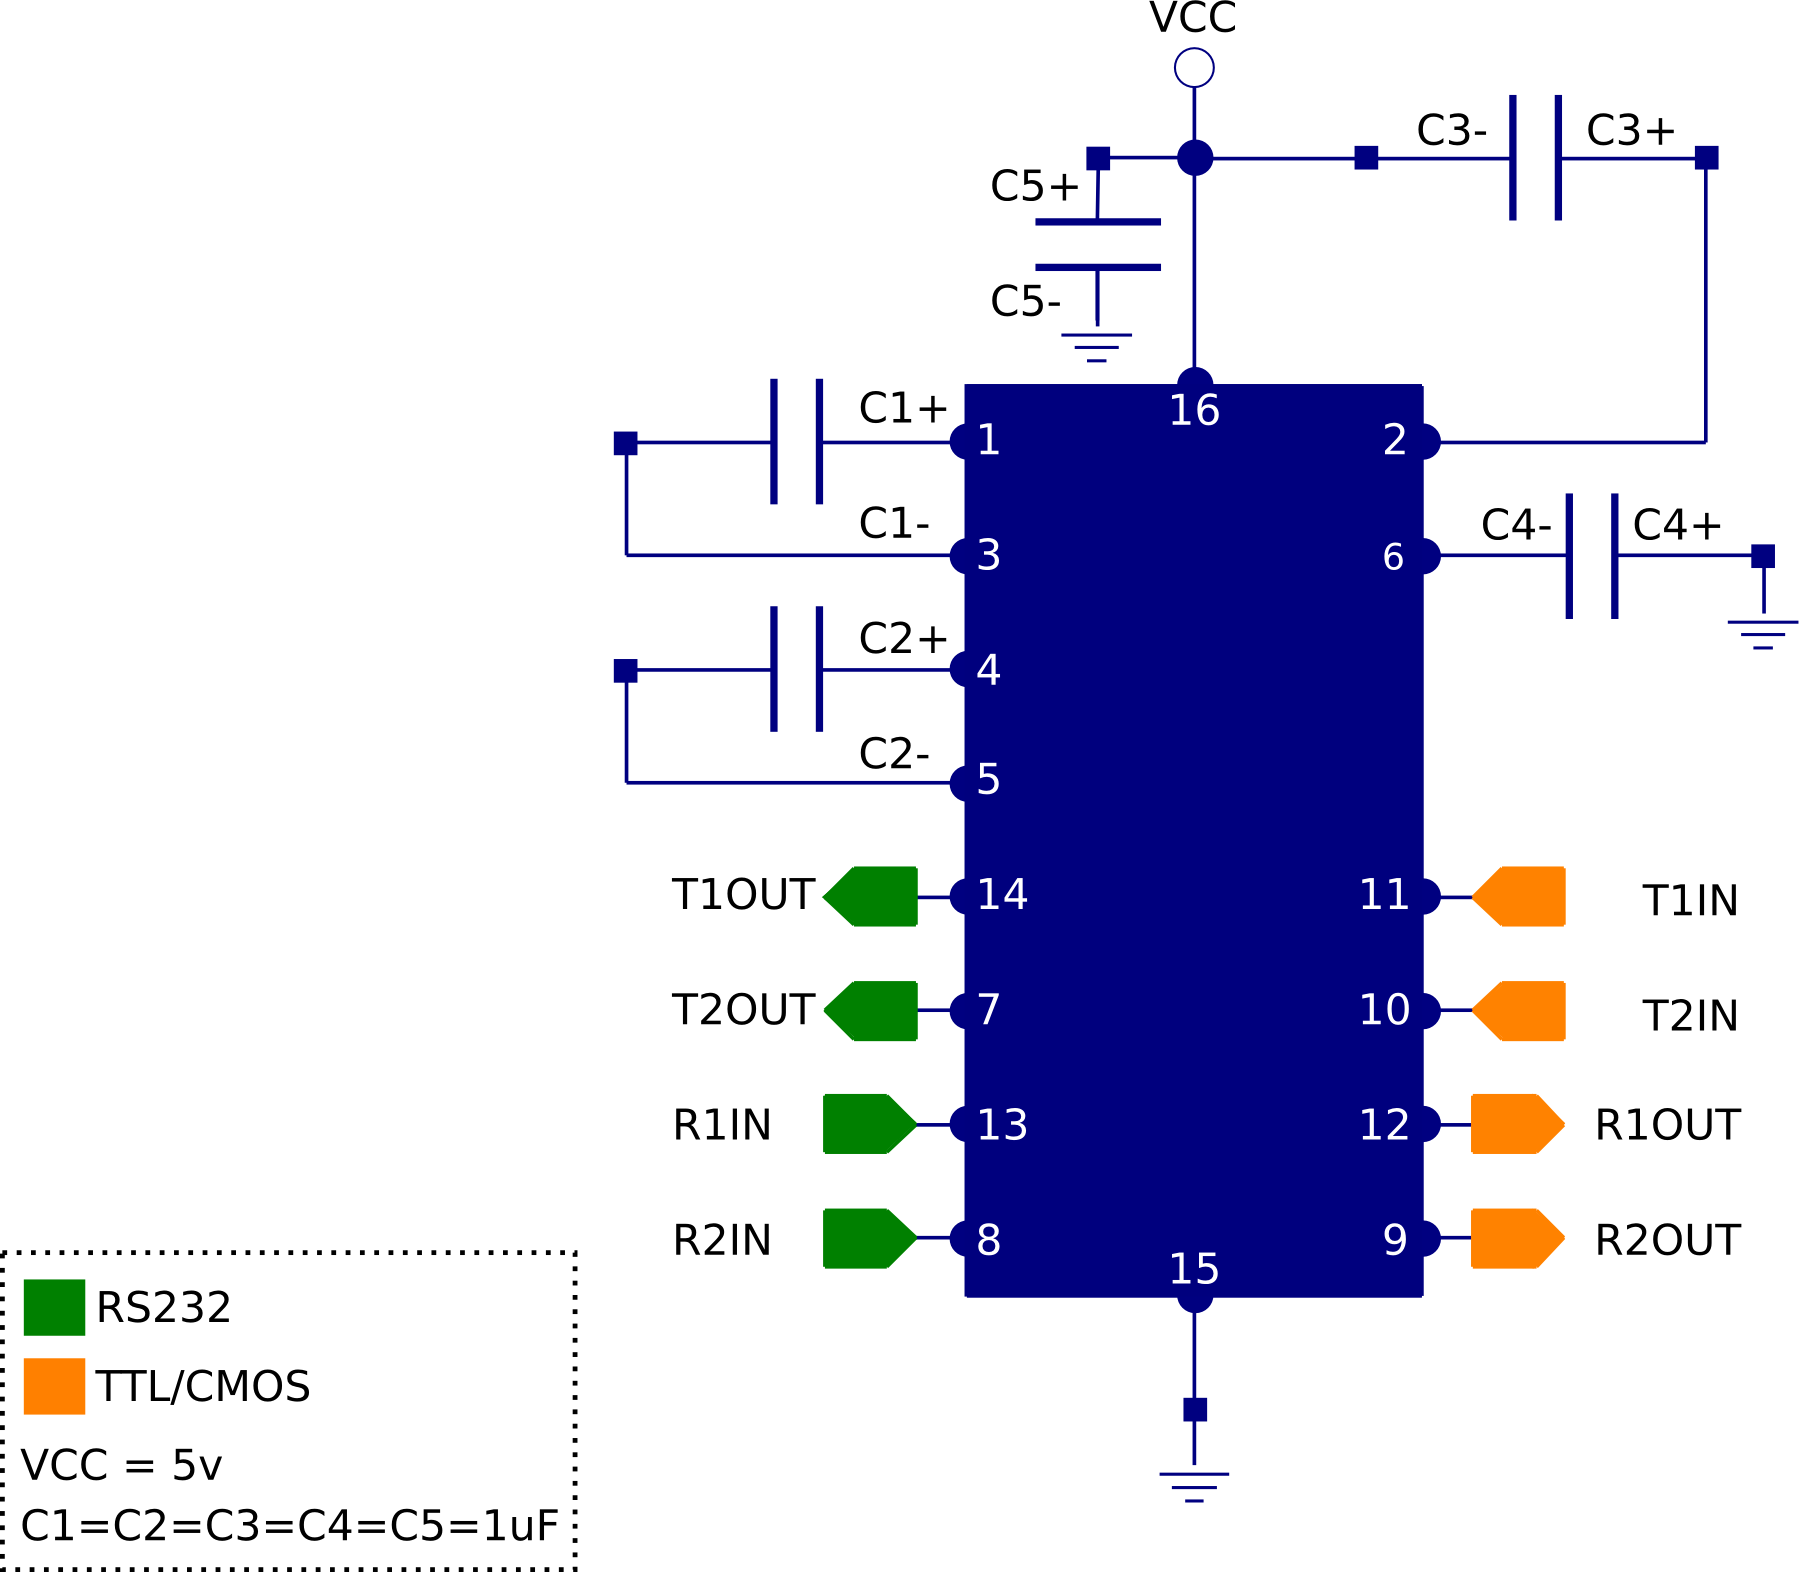
\includegraphics[width=300pt]{./images/esq_max232.png}
\caption{Esquema de conexionado del circuito integrado MAX232.}
\label{fig:esq_max232}
\end{figure}

\subsection{Formato de la trama}
\label{subsec:trama}

La norma RS232 comprende varios protocolos de entre los cuales cabe destacar la diferenciación entre \textit{síncronos} y \textit{asíncronos}. Los primeros requieren el uso de una señal de reloj que, gestionada por el maestro en la comunicación, sirve para sincronizar el envío de datos entre los componentes. En el caso de los asíncronos la transmisión se basa en el determinación de la temporización a ambos lados, de forma que se puede utilizar una sola línea modificando los datos con una frecuencia acordada.  Debido a que el número de conectores suele ser un bien preciado en los microcontroladores, se ha optado por utilizar una comunicación asíncrona, reduciendo de tres a dos el número de contactos necesarios para una comunicación unidireccional.

Atendiendo al protocolo establecido por la norma RS232 para las comunicaciones asíncronas sin tiempo de inicio preestablecido, la información se envía, como ilustra la figura \ref{fig:trama_rs232}, estructurada en cuatro partes:

\begin{itemize}
	\item{START: bit de inicio o arranque. Inicia la comunicación cuando la línea, que en estado de reposo se encuentra en un uno lógico, pasa a un cero lógico. A partir de este flanco, el receptor comienza a leer las señales con una frecuencia preestablecida.}
	\item{DATA: bits de datos. Se envía el número de bits preestablecido, empezando por el de menor peso, LSB (\textit{Least Significant Bit}), y terminando por el de mayor peso, MSB (\textit{Most Significant Bit}).}
	\item{PARITY: bit de paridad. Si se ha preestablecido la transmisión de un bit de paridad para comprobar la integridad de los datos, se enviará un uno o un cero lógico en función del tipo de paridad (par o impar) y la palabra enviada.}
	\item{STOP: bit de parada. La línea se mantiene en un uno lógico cuando termina la transmisión. Este bit, que puede mantenerse el equivalente a 1, 1.5 o 2 bits, indica la finalización de la transmisión.}
\end{itemize}

\begin{figure}[!htp]
\centering
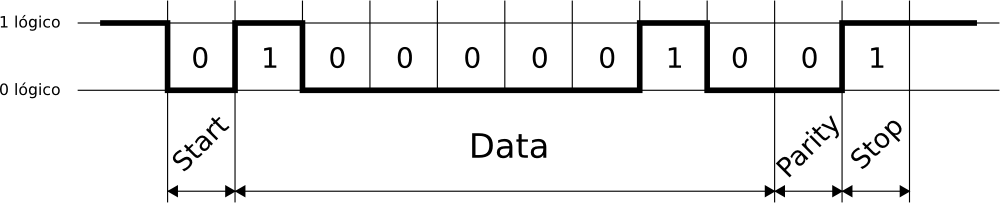
\includegraphics[width=300pt]{./images/trama_rs232.png}
\caption[Ejemplo de envío de una trama según RS232]{Ejemplo de envío de una trama según RS232. Código ASCCI de ``A'' (01000001), 8 bits de dato con paridad par y 1 bit de stop.}
\label{fig:trama_rs232}
\end{figure}

Dado que los datos a transmitir serán de tipo char y la integridad de los datos no resulta crítica, en este proyecto se ha optado por implementar una comunicación con un bit de start, ocho bits de dato, ninguno de paridad y un bit de stop. Éstos serán los datos a tener en cuenta por la aplicación que transmita los datos desde el ordenador, y la configuración del receptor del microcontrolador.

\subsection{Velocidad de transmisión}

La unidad más utilizada para expresar la velocidad de transmisión, la cantidad de información enviada, es el \textit{baudio} \cite{baudio}. Proporcional a los bits por segundo (bps), expresa el número de bits de información. La velocidad a la que pueden trabajar tanto los puertos serie de un ordenador como los microcontroladores está normalizada a 75, 150, 300, 600, 1200, 2400, 4800, 9600 baudios, etc.\cite{pic_serie}.

Para la aplicación que nos ocupa, se ha escogido una velocidad de transmisión de 19200 baudios. Si bien podrían utilizarse velocidades mayores, nuestro sistema no requiere una alta velocidad de transmisión y este valor facilita los cálculos para la configuración del microcontrolador, como se analizará en la sección correspondiente.
